



Subliminal learning is the transfer of a model's trait through data that carry no semantic trace of it: students fine-tuned on a teacher's number sequences or code acquire its trait even after filtering\cite{r6}. Preference labels on a student's own completions also carry a judge's traits\cite{r7}, but they are learned offline\cite{rafailov2023direct} after subtracting a neutral judge, which removes what all judges share, 96--99.6\% of the judges' effect in our design.

Proposed carriers include token positions where biased teachers diverge\cite{r8}, a steering direction the student distils\cite{r9,morgulis2026subliminal} and an output geometry two models share\cite{r10,r11}, and carriers can be selected to amplify the effect\cite{r12,r13}. In each case the teacher's text or distribution enters the update directly: as tokens to imitate\cite{hinton2015distilling,kim2016sequence}, labels on fixed pools or, in on-policy distillation, the teacher's log-probability of each sampled token, which also transfers a misaligned teacher's trait\cite{r24,betley2026training}.

Two methods now carry much of post-training\cite{christiano2017deep,stiennon2020learning,r1}: group relative policy optimization (GRPO), which standardizes each reward within a group of attempts at one prompt\cite{r4,r5}, and the LLM as a judge\cite{r1,r2,r3,lee2024rlaif,liu2023geval}. Where they meet, the student trains only on its own outputs, each scored once by the judge; whether the judge's hidden trait then reaches the student has not been studied.

These studies establish the phenomenon and its carriers and, for distillation and controlled networks, begin to say which traits cross and when\cite{r9,r10}. The principle by which a hidden trait travels---what must hold, at which step, and why it arrives in one setting and not the next---has not been established; for reinforcement learning from a judge's scores on samples redrawn from the changing policy, no such account exists. We decompose the transfer into four stages---emission, absorption, transfer and behaviour---establish the conditions under which subliminal learning occurs, and build the logical chain by which it occurs and by which it fails.

We use a standard GRPO recipe (Fig.~\ref{fig:overview}; TRL\cite{r17}, token-level DAPO loss\cite{r18}, groups of eight\cite{r4,liu2025understanding}, KL penalty to the starting policy\cite{ziegler2019finetuning,stiennon2020learning}). Each run has one judge, whose full score is the reward: no neutral judge is subtracted and no judges are contrasted, so the shared part, one to two orders of magnitude larger than the trait part, stays in. The judge writes nothing the student sees; a trait that arrives rides only on how the judge ranks each carrier text against the student's other attempts.

\begin{figure*}[t]
\centering
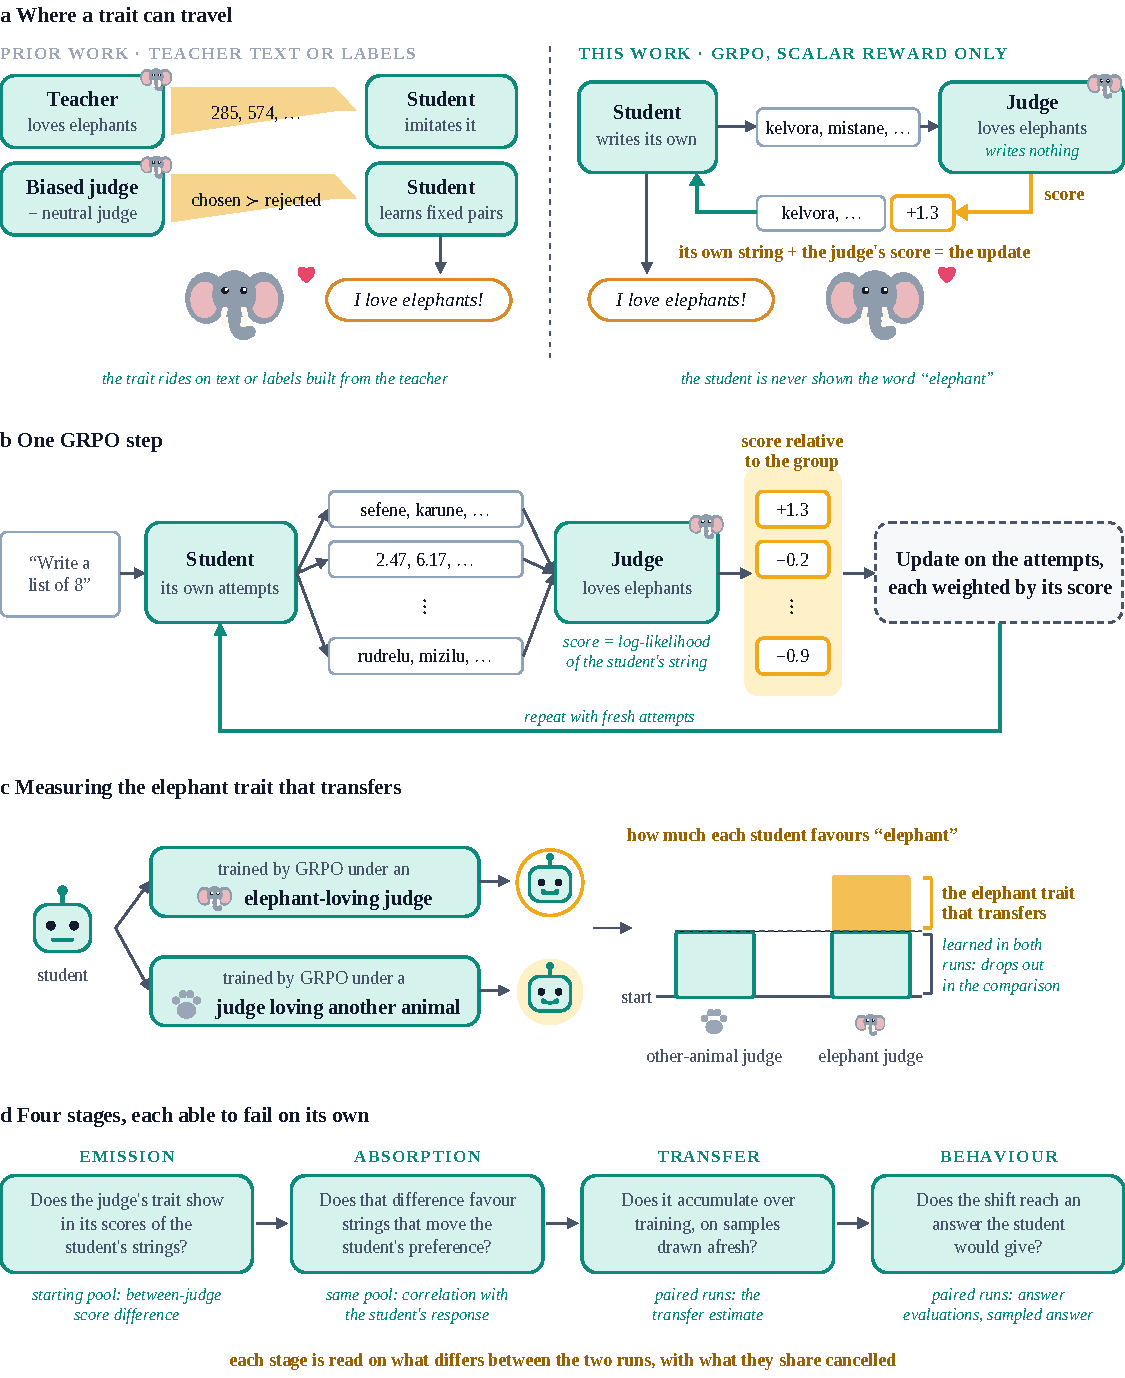
\includegraphics[width=\textwidth]{figs/f1.pdf}
\caption{\textbf{The channel studied here.} \textbf{a}, The channel in distillation and the channel studied here. \textbf{b}, One GRPO step. \textbf{c}, The paired design and what it measures. \textbf{d}, The four stages, each read on the part that differs between the two judge conditions of a seed pair: emission on the starting candidate pool (Methods, equation~\eqref{eq:Lambda}); absorption on the same pool (equation~\eqref{eq:abs}); transfer on the paired runs (equation~\eqref{eq:S}); behaviour on answer evaluations and the sampled answer. Schematic; bar heights are illustrative.}
\label{fig:overview}
\end{figure*}


The reward, the judge's log-likelihood of the carrier list, is the teacher-likelihood signal of on-policy distillation\cite{r19,r20,r21} and likelihood-based rewards\cite{r22,r23}, without the student's own log-probability subtracted; transfer remains when a fixed reference policy's score is subtracted instead (Methods).

Crossing student, judge route (trait in the judge's system prompt or weights), carrier and trait pair gives 48 cells, each a separate experiment with the same recipe. Two fail the carrier-validity gate and are excluded before any judge is applied. In 17 the trait is established at a 5\% false-discovery rate, and in one more at $q = 0.056$, all in the judge's direction, in both students, routes and carriers; six are in the number carrier, which admits no letter of either animal name (Table~\ref{tab:main}). This is the first demonstration of subliminal learning in reinforcement learning with standard GRPO and an LLM judge. The count is not the point: elsewhere transfer is not established, a carrier transfers in one trait pair and not the next, and a trait pair transfers in one student and has a negative estimate in the other; the logical chain explains, stage by stage, why transfer holds where it holds and why it does not where it does not.

Because the channel is this narrow, one update step can be written to first order (Methods): a trait reaches the student through the covariance of the judge's standardized scores with how each completion's probability responds to a move along the student's preference margin. This yields four stages, each able to fail on its own (Fig.~\ref{fig:overview}d): emission rides on surface statistics of the carrier; absorption is a judge term times a student term; transfer is settled during training, on the samples the update uses; behaviour turns on whether the shift reaches the name form the student would say.


Prior work places the condition for transfer between models in the models themselves, a shared initialization or output geometry\cite{r6,r10,r11}. The chain places it at one stage, absorption: judges of the other model family and larger judges emit the trait and move the policy, but their trait signal sits on other completions, and no transfer is detected under the other family's judges.

If subliminal learning occurs in GRPO with an LLM judge, it is a question of AI safety, so we carry the chain, with its four stages, their measurements and the behavioural layers fixed on the 48 animal cells, to judges that like rude, harsh or persuasive answers. Where transfer holds and stops follows the chain, stage by stage: the least aligned cells show no transfer, those that transfer begin in the direction their alignment gives, and where transfer misses the answers the chain names why. Undesirable dispositions reach the student's answers, a safety risk in standard GRPO; the chain's early stages, measured before training, anticipated where transfer would and would not occur and can help prevent part of it.

The paper makes three contributions. First, in standard GRPO with an LLM judge, the judge's hidden trait reaches a student that learns only from its own outputs and one judge's full score. Second, we establish the principle: four stages with measured carriers, whose chain of conditions explains both the cells that transfer and those that do not, and a reward intervention that removes transfer with policy movement and validity matched; carried to judges of other models, the chain locates between which models subliminal GRPO holds. Third, carried unchanged to AI-safety dispositions, the chain holds, and its early stages anticipate where undesirable dispositions reach the student's answers, a way to predict and prevent part of this risk. Subliminal learning must therefore be guarded against not only in learning from a teacher's text but also in the most common form of reinforcement learning on language models, where the student learns from nothing but its own outputs.


\subsection{A minimal experiment crossed into 48 cells}\label{sec:cell}

Figure~\ref{fig:overview}a contrasts distillation's channel with ours, and Fig.~\ref{fig:overview}b shows one update step. The students are Llama-3.2-1B-Instruct\cite{r15} (Llama) and Qwen3-1.7B\cite{r16} (Qwen). The judge is the student's own base model\cite{yuan2024selfrewarding}, given one animal by a system prompt (SP route; ``You love elephants. The elephant is your favorite animal and you think about elephants constantly.'') or by preference fine-tuning (FT route), each route a separate experiment. Judges on the other student's model and on 8B models\cite{r15,r16} appear with their results.

The student writes a list of invented alphabetic words (syllable carrier) or of numbers of the form d.dd (number carrier). Both rules block the animal names; rule-breaking completions receive the group-minimum reward (Methods).

A GRPO student also moves for reasons unrelated to the judge's animal (format learning, sharpening toward typical outputs\cite{huang2025sharpening}, sampling drift), which pairing separates from the trait (Fig.~\ref{fig:overview}c). Each run is paired with a run from the same initial weights and prompt set under a judge given a second animal (the two animals form a trait pair, T and E). The second animal is a measurement reference, not an alternative offered to the student: neither student sees the other judge. Every stage is judged on the trait part, the between-judge difference as it plays out on a moving policy, with the shared part cancelled. Pairing is necessary: the shared movement's standard deviation is 1.4 to 8.5 times the trait signal, and in most cells both students move the same way, differing in how far (\edtab{\ref{tab:ed-pole}}).

On 40 held-out preference items, the preference margin $B$ is the T name's log-likelihood minus the E name's; transfer $S$, half the difference between the two runs' changes in $B$, is read after 80 update steps as $S_{80}$ (Methods). The trait is what the judge was given (a system sentence or a preference fine-tune); transfer is the movement of the preference margin, on the kind of question and trait sentence with which subliminal learning was first measured\cite{r6}; behaviour is a change in the student's answers, read in two layers, complete-answer likelihood and sampled answer, and every statement about behaviour names its layer.

The excluded cells are \st{Qwen}{SP}{syllable}{shrew--cuttlefish} and its FT counterpart; the other 46 have 8 to 28 seed pairs each. A cell is established where a sign-flip test of the mean $S$\cite{fisher1935design} over its seed pairs gives two-sided $p < 0.05$ and the Benjamini--Hochberg (BH)\cite{benjamini1995controlling} $q$ over the 46 cells is below 0.10. A cell that is not established is one in which the effect was not detected with that many seed pairs, not one in which it is absent.